\documentclass[11pt,a4paper]{report}
\usepackage[utf8]{inputenc}
\usepackage[french]{babel}
\usepackage[T1]{fontenc}
\usepackage{amsmath}
\usepackage{amsfonts}
\usepackage{amssymb}
\usepackage{xcolor}
\usepackage{gensymb}

\usepackage{geometry}
\geometry{hmargin=2.5cm,vmargin=1.5cm}
\usepackage{wasysym}
\usepackage{graphicx}

\author{Mathieu Sarrat}
\title{LC15 - Cinétique homogène}

\makeatletter
\renewcommand{\thesection}{\@arabic\c@section}
\makeatother


\begin{document}
\maketitle

\section*{Niveau, Pré-requis et objectifs}
\begin{itemize}
	\item \textbf{Niveau :} MPSI\\
	
	\item \textbf{Pré-requis :}
	\begin{itemize}
		\item Oxydoréduction,
		\item Dosage par suivi spectrophotométrique,
		\item Loi de Beer-Lambert,
		\item Équations différentielles.\\
	\end{itemize}
	
	\item \textbf{Objectifs :}
	\begin{itemize}
		\item Définir la vitesse d'une réaction chimique et la lier aux concentrations (ou à 					l'avancement dans un cadre d'étude simplifié.)
		\item Lorsqu'une réaction admet un ordre, définir ordre global et ordres partiels.
		\item Introduire l'énergie d'activation et loi d'Arrhénius, signification. 
		\item Introduire des méthodes de suivi et de détermination des ordres de réaction.
		\item Exploiter une méthode de suivi cinétique.\\
	\end{itemize}
		
	\item \textbf{Recommandations :}
	\begin{itemize}
		\item Attention au réglage en longueur d'onde du spectro, pour ne pas le saturer (il est 				peut-être préférable de ne pas se placer à la longueur d'onde d'absorption maximale).
		\item Retourner un bêcher par-dessus une solution d'ions iodure préparée à l'avance, car le 			dioxygène de l'air peut oxyder ces ions.
		\item Cuves en verre pour le spectro, à cause de la propanone qui attaque le plastique.\\
	\end{itemize}
	
	\item \textbf{Liste du matériel :}
	\begin{itemize}
		\item spectrophotomètre UV-visible, de préférence thermostaté et avec port USB;
		\item \textbf{cuves de spectro en verre} (l'acétone attaque le plastique);
		\item ordinateur portable avec Latis Pro et souris;\\
		\item acétone à 2 mol/L et à 1 mol/L (cela fonctionne aussi avec de la propanone pure car 			on aura $\simeq$ 5.35 mol/L une fois dans les 50 mL de milieu réactionnel);
		\item acide chlorhydrique à 0.1 mol/L et à 0.05 mol/L;
		\item solution de $I_2$ (à $10^-4$ mol/L) dans KI (100 g/L d'eau);
	\end{itemize} 
\end{itemize}

\newpage
\section*{Introduction}

Nous avons vu dans les leçons précédentes, en début d'année, qu'une réaction chimique correspond
à la transformation d'un système chimique depuis un état initial donné (caractérisé par une certaine valeur du quotient réactionnel) vers un état final, caractérisé par la consommation totale d'un réactif ou par l'existence d'un équilibre (constante d'équilibre). Jusque là nous ne nous sommes intéressés qu'à ces états, \textbf{sans se préoccuper de comment le système chimique passait de l'un à l'autre}.\\  

\textbf{Le facteur temps est notamment absent de cette approche}, or toutes les réactions chimiques ne se font pas instantanément, certaines étant bien plus rapides que d'autres :\\

\textcolor{red}{\textbf{Manip à la flexcam}
\begin{itemize}
	\item Réaction n$\degree$1. Bécher contenant des ions $\text{Fe}^{2+}$, bécher contenant 10 mL 		d'ions $\text{MnO}_4^-$, $\text{H}^+$ (permanganate acidifié);
	\item Réaction n$\degree$2. Bécher contenant de l'acide oxalique, bécher contenant 10 mL d'ions 
	$\text{MnO}_4^-$, $\text{H}^+$ (permanganate acidifié);
	\item Verser en même temps le permanganate dans les deux béchers, sous la flexcam. Constater 		que la première réaction est quasiment instantanée alors que la seconde ne semble même pas 			avoir lieu.\\
\end{itemize}}

Écrivons les équations des deux réactions que nous venons de présenter :
\begin{itemize}
	\item \textbf{Réaction n$\degree$1 :} couples $\text{Fe}^{3+}/\text{Fe}^{2+}, 
	E\degree = 0.77\;V$ et $\text{MnO}_4^-/\text{Mn}^{2+}, E\degree = 1.51\;V$
	\begin{equation}
		\boxed{\text{MnO}_4^- + 8\text{H}^+ + 5\text{e}^- = \text{Mn}^{2+} + 4\text{H}_2\text{O}}
		\quad\text{et}\quad \boxed{\text{Fe}^{3+} + \text{e}^- = \text{Fe}^{2+}}		 
	\end{equation}
	d'où la réaction
	\begin{equation}
		\boxed{\text{MnO}_4^- + 5\text{Fe}^{2+} + 8\text{H}^+ 
		= 5\text{Fe}^{3+} + \text{Mn}^{2+} + 4\text{H}_2\text{O}}
	\end{equation}
	\item \textbf{Réaction n$\degree$2 :} couple 
	$\text{CO}_{2,(g)}/\text{H}_2\text{C}_2\text{O}_{4,(aq)}, E\degree = -0.44\;V$ 
	\begin{equation}
		\boxed{2\text{CO}_{2,(g)} +2\text{H}^+ + 2\text{e}^-
		= \text{H}_2\text{C}_2\text{O}_{4,(aq)}}
	\end{equation}
	d'où la réaction
	\begin{equation}
		\boxed{2\text{MnO}_4^- + 5\text{H}_2\text{C}_2\text{O}_{4,(aq)} + 6\text{H}^+ 
		= 2\text{Mn}^{2+} + 10\text{CO}_{2,(g)} + 8\text{H}_2\text{O}}
	\end{equation}
\end{itemize}
Si on compare les potentiels standard des couples rédox en contact, on se rend compte que la réaction est thermodynamiquement favorable, mais cela ne nous dit absolument rien sur la vitesse de cette réaction.

La \textbf{cinétique chimique consiste à mesurer puis à modéliser l'évolution temporelle d'un système chimique considéré} entre les états initiaux et finaux. Cette étude peut se faire selon deux points de vue :
\begin{itemize}
	\item un \textbf{point de vue macroscopique}, consistant à introduire des lois de vitesse permettant de savoir à quel rythme les réactifs sont consommés et les produits formés,
	\item un point de vue microscopique, correspondant à l'interprétation de l'équation bilan en termes d'actes élémentaires plus ou moins rapides et qui ensemble forment un mécanisme plus ou moins complexe.\\
\end{itemize}

La cinétique chimique a une importance considérable : elle fournit un cadre pour décrire à la fois des réactions qui s'emballent (conduisant à des explosions) et des phénomènes bien plus lents comme la formation de rouille sur des structures en fer laissées sans protection. Elle nous permet d'expliquer pourquoi placer des aliments dans un réfrigérateur ou dans un congélateur permet d'accroître leur durée de conservation, et nous donne des clés pour essayer d'optimiser des procédés chimiques industriels. Dans ce cas, l'objectif est d'obtenir un bon rendement le plus rapidement possible, tout en minimisant la consommation d'énergie et le gaspillage d'atomes. Cette discipline a donc, conjointement avec la thermodynamique, une grande importance dans le milieu industriel.

\newpage
\section{Modélisation cinétique d'une réaction chimique}\label{sec:1}

Dans cette partie, nous allons nous appuyer sur la réaction entre les ions permanganate et les ions ferreux. On veut définir une vitesse pour la réaction chimique. Nous allons formuler plusieurs hypothèses :
\begin{itemize}
	\item le système est \textbf{fermé} : la matière ne quitte pas le récipient dans lequel se fait la réaction;
	\item le système est \textbf{homogène} : tous les constituants sont présents dans la même phase (gaz ou solution), la concentration est la même en tout point du milieu réactionnel.
	\item l'évolution est \textbf{isochore et isotherme} : on travaille à volume et température constants.
\end{itemize}

\subsection{Vitesse de réaction}

Faire le tableau d'avancement de la réaction n$\degree$1. On peut commencer par évaluer le taux d'évolution des concentrations en produits et en réactifs, ce qui implique de calculer les dérivées temporelles de ces concentrations :
\begin{equation}
	v(\text{MnO}_4^-) = - \frac{d}{dt}[\text{MnO}_4^-] \quad\text{est la vitesse de disparition des ions permanganate},
\end{equation}
et
\begin{equation}
	v(\text{Fe}^{3+}) =  \frac{d}{dt}[\text{Fe}^{3+}] \quad\text{est la vitesse de formation des ions ferriques}.
\end{equation}
Commentons ces expressions :
\begin{itemize}
	\item $1\degree)$ : on veut des vitesses positives, d'où le signe - 
				devant la vitesse de disparition;
	\item $2\degree)$ : l'unité de ces vitesses est le $\text{mol}.\text{L}^{-1}.\text{s}^{-1}$;
	\item $3\degree)$ : ces vitesses peuvent être différentes pour chaque espèce, ce qui n'est pas pratique pour caractériser une réaction.\\
\end{itemize}

Le tableau d'avancement nous permet de remarquer que toutes les quantités de matière (et donc les concentrations) à chaque instant sont données sans ambiguïté pourvu que l'on connaisse l'avancement réactionnel (variable de De Donder) et les coefficients stœchiométriques intervenant dans la réaction. On va donc utiliser l'avancement (l'avancement volumique $x$ puisqu'on travaille à volume constant) pour définir la \textbf{vitesse volumique globale de réaction} :
\begin{equation}
	v \equiv \frac{dx}{dt}, \quad\text{en}\;\text{mol}.\text{L}^{-1}.\text{s}^{-1}.
\end{equation}

Relions maintenant cette vitesse aux concentrations en chaque espèce, en nous appuyant sur le tableau d'avancement. On a par exemple \textcolor{red}{(poser le calcul au tableau)}
\begin{equation}
	[\text{MnO}_4^-](t) = [\text{MnO}_4^-]_0 - x(t) \quad\text{et}\quad
	[\text{Fe}^{3+}](t) = [\text{Fe}^{3+}]_0 + 5x(t),
\end{equation}
d'où, en dérivant par rapport au temps 
\begin{equation}
	\frac{d}{dt}[\text{MnO}_4^-] = -\frac{dx}{dt} = -v, \quad\text{d'où}\quad
	v = -\frac{d}{dt}[\text{MnO}_4^-]
\end{equation}
et, de même,
\begin{equation}
	\frac{d}{dt}[\text{Fe}^{3+}] = 5\frac{dx}{dt} = 5v, \quad\text{d'où}\quad
	v = \frac{1}{5}\frac{d}{dt}[\text{Fe}^{3+}].
\end{equation}

On généralise : pour une réaction du type
\begin{equation}
	\sum_i \nu_i X_i = 0,
\end{equation}
$X_i$ désignant une espèce chimique participant à la réaction et $\nu_i$ le \textbf{nombre stœchiométrique algébrique} figurant dans l'équation bilan, positif pour un produit et négatif pour un réactif, on a la relation suivante entre vitesse globale de réaction et concentration en $X_i$
\begin{equation}
	\boxed{v = \frac{1}{\nu_i}\frac{d}{dt}[X_i]}.
\end{equation}
Le nombre stoechiométrique étant algébrique, positif pour un produit, négatif pour un réactif, \textbf{cette vitesse est positive si la réaction évolue dans le sens direct}.

\subsection{Facteurs cinétiques}

Il est possible de modifier la rapidité d'une réaction en agissant sur un certain nombre de paramètres, contrôlables expérimentalement. \textbf{On appelle facteur cinétique tout paramètre influençant la vitesse de réaction chimique.}

\subsubsection{Influence de la température (MANIP)}

Prendre 3 couples de tubes à essais. Dans chaque couple, le premier tube contient KI avec $H^+$ (acide sulfurique), le second tube contient de l'eau oxygénée. Les concentrations et volumes sont identiques.
\begin{itemize}
	\item Couple n$\degree$1 : plongé dans un bain eau/glace
	 
	\item Couple n$\degree$2 : laissé à température ambiante
	
	\item Couple n$\degree$3 : plongé dans un bain thermostaté à 40$\degree$C
\end{itemize}

\textbf{Apparition d'une coloration jaune, liée à la formation de l'ion triiodure $I_3^-$} (complexe entre $I_2$ et $I^-$ parfois noté $I_{2,(aq)}$, selon la réaction d'oxydoréduction suivante
\begin{equation}
\boxed{\text{H}_2\text{O}_{2\text{(aq)}} + 2 \text{I}^{-}_\text{(aq)} + 2 \text{H}^+_\text{(aq)} 
= I_{2\text{(aq)}} + 2\text{H}_2\text{O}_\text{(l)}},
\end{equation}
avec $E\degree(\text{I}^2/\text{I}^-) = 0.54$ V et $E\degree(\text{H}_2\text{O}_{2}/\text{H}_2\text{O}) = 1.78$. \textbf{Plus la température est élevée}, plus la coloration jaune apparaît vite, traduisant une formation plus rapide de triiodure et donc une \textbf{vitesse de réaction plus grande}.

\subsubsection{Influence de la concentration d'un réactif (MANIP)}

\begin{itemize}
	\item Soit 2 béchers contenant 15 mL d'eau oxygénée à $0,01 mol/L$ (éprouvette) et 5 gouttes 		d'acide sulfurique à 1 mol/L,
	\item Soit 2 béchers contenant une solution de KI ($0.1 mol/L$) avec eau distillée
		\begin{itemize}
			\item Bécher 1 : 10 mL de KI, 25 mL d'eau distillée (éprouvette)
			\item Bécher 2 : 20 mL de KI, 15 mL d'eau distillée (éprouvette). 
		\end{itemize}
\end{itemize}
Mélanger simultanément. Observer. La réaction va plus vite (apparition de la coloration) dans le deuxième bécher, contenant plus d'ions iodure. La couleur finale est la même dans les 3 béchers : la même quantité de matière finale d'ions triiodure a été formée. On en conclut que la réaction évolue d'autant plus vite que la concentration est forte, donc \textbf{la vitesse augmente avec la concentration}.

\subsubsection{Présence d'un catalyseur}

On a vu au lycée la notion de catalyse : l'ajout de certaines espèces chimiques, appelées catalyseurs, augmente la vitesse de réaction. La réaction de synthèse de l'ammoniac, à partir du dihydrogène et du diazote est catalysée par le fer et la potasse : 
\begin{equation}
	\text{N}_{2(g)} + 3\;\text{H}_{2(g)}  \rightleftarrows 2\;\text{NH}_{3(g)} 
\end{equation}
Les réactions chimiques intervenant dans le processus de digestion sont catalysées par des enzymes.\\

Un catalyseur est intégralement reconstitué durant une réaction chimique : il est consommé à un moment donné puis produit à nouveau. Un catalyseur ne peut qu'accélérer une réaction thermodynamiquement possible, et ce \textbf{sans effet sur la composition à l'état final}.

\subsubsection{Interprétation microscopique}

Si on estime qu'une réaction chimique se produit lorsqu'il y a collision entre deux molécules de réactifs, on comprend intuitivement que
\begin{itemize}
	\item plus la température est élevée, plus les réactifs ont d'énergie ce qui \textbf{favorisant la probabilité d'un choc efficace} (c'est à dire capable de briser une liaison) entre deux molécules de réactifs;
	\item plus la concentration est élevée, plus la probabilité de choc entre deux réactifs est 		élevée;
\end{itemize}

\subsection{Loi de vitesse et ordre de réaction}

Nous avons vu que la concentration en réactifs était un facteur cinétique, tout comme la température. On appelle \textbf{loi de vitesse} une expression mathématique reliant la vitesse globale de réaction à la température et aux concentrations en réactifs et catalyseurs.\\

Considérons la réaction d'iodation de la propanone, catalysée par les ions $\text{H}^+$ :
\begin{equation}
	\text{C}_3\text{H}_6\text{O} + \text{I}_2 \xrightarrow{H^+} 
	\text{C}_3\text{H}_5\text{O}\text{I}^- + \text{I}^- + \text{H}^+
\end{equation}

On dit que cette réaction \textbf{admet un ordre} si et seulement si sa loi de vitesse a la forme suivante :
\begin{equation}
	\boxed{v = k(T)[\text{C}_3\text{H}_6\text{O}]^\alpha [\text{I}_2]^\beta [\text{H}^+]^\gamma}.
\end{equation}

Dans cette expression, \textbf{qui est un modèle}
\begin{itemize}
	\item $\alpha$, $\beta$ et $\gamma$ désignent les \textbf{ordres partiels} relatifs à la propanone, au diiode et aux ions oxonium respectivement;
	\item $\alpha + \beta + \gamma$ est \textbf{l'ordre global} de la réaction;
	\item $k(T)$, \textbf{constante de vitesse} est fonction de la température (et éventuellement d'autres facteurs cinétiques comme la pression pour les gaz ou pouvoir dispersant du solvant pour la production d'ions...), permettant ainsi de séparer la dépendance en température de la dépendance en concentration. Son unité dépend de l'ordre global, on s'arrange pour que la vitesse soit exprimée en mol/L/s.
	\item la \textbf{concentration en catalyseur intervient dans la loi de vitesse}.
\end{itemize}

\subsection{Loi d'Arrhénius (1889)}

En 1889, le chimiste suédois Arrhenius a proposé une loi empirique permettant de relier la loi de vitesse à la température en fournissant une expression pour la constante de vitesse :
\begin{equation}
	k(T) = A\text{exp}\left(-\frac{E_A}{RT}\right),
\end{equation}
où $R$ désigne la constante des gaz parfaits et $T$ la température. Cette loi restitue le comportement qualitatif que nous avions mis en évidence plus tôt, à savoir que la vitesse de réaction augmente si la température augmente.\\

La grandeur $E_A$ est appelée \textbf{énergie d'activation de la réaction}, généralement de plusieurs dizaines à quelques centaines de $kJ.mol^{-1}$ de réactifs. Elle est un \textbf{ordre de grandeur de l'énergie nécessaire pour qu'un choc entre deux molécules soit efficace} (bonne orientation) et puisse conduire à la rupture et à la formation des liaisons entre atomes. Ainsi, une réaction sera d'autant plus lente que son énergie d'activation sera élevée, car la probabilité qu'une molécule ait une énergie suffisante pour générer un choc efficace sera de plus en plus faible.\\

$A$ est le \textbf{facteur pré-exponentiel}, tenant compte de la fréquence des collisions entre molécules ainsi que des effets liés à l'encombrement et à la géométrie des molécules.\\

On peut déterminer expérimentalement ces deux quantités, en effectuant la même réaction, avec des concentrations initiales identiques en espèces chimiques, mais à plusieurs températures différentes. Le tracé de 
\begin{equation}
	\text{ln}\;k = f\left(\frac{1}{T}\right)
\end{equation}
conduit à une droite de pente $\frac{-E_A}{R}$ et d'ordonnée à l'origine $\text{ln}\;A$ (avec une grosse incertitude pour $A$ du fait du logarithme) si la réaction suit la loi d'Arrhenius. Attention, comme $E_A$ et $A$ dépendent faiblement de la température, la loi d'Arrhenius n'est généralement valable que sur un intervalle donné de températures.\\

Cette loi a pu être vérifiée expérimentalement pour un grand nombre de réactions chimiques, mais elle n'est pas infaillible : les réactions enzymatiques ne la suivent pas, par exemple.


\section{Étude expérimentale de la iodation de la propanone}\label{sec:2}

L'ordre de réaction est une \textbf{notion purement expérimentale} et l'un des buts de la cinétique chimique est de \textbf{déterminer les ordres partiels} de réactions par rapport à tous les réactifs, \textbf{ainsi que la constante de vitesse} à une température donnée. Il nous faut pour cela \textbf{mesurer au cours du temps la concentration de chaque espèce intervenant dans le modèle de loi de vitesse}.

\subsection{Suivi cinétique \textcolor{red}{(manip au fur et à mesure)}}

Il existe plusieurs méthodes pour effectuer un suivi cinétique en chimie.

On dispose tout d'abord de méthodes chimiques, reposant sur un \textbf{titrage}. On peut prélever à intervalles de temps régulier des \textbf{échantillons de volume négligeable mais connu avec précision} du milieu réactionnel (celui-ci doit être bien homogène), puis leur faire subir une \textbf{trempe chimique}. Ceci consiste à diluer l'échantillon dans un volume d'eau froide bien plus important, connu lui aussi, \textbf{réduisant ainsi brutalement température et concentration}. Ceci met un coup d'arrêt à la réaction et permet à l'expérimentateur de doser tranquillement ses échantillons. L'inconvénient de ces méthodes est qu'elles sont lourdes à mettre en pratique (plusieurs dosages) et destructives : on agit sur le milieu réactionnel, ce qui vient parasiter la réaction que l'on souhaite étudier.\\

Il existe ensuite des méthodes physiques, moins perturbatrices, qui consistent à mesurer une grandeur dépendant de la concentration des espèces intervenant dans la réaction :
\begin{itemize}
	\item lorsqu'un \textbf{gaz} est dégagé, on peut procéder par \textbf{manométrie} et mesurer la 	pression. Si on travaille à volume et température constants, on peut remonter à la quantité de 		matière de gaz par la loi des gaz parfaits, par exemple;
	\item lorsque des \textbf{ions} sont impliqués, on peut utiliser la \textbf{conductimétrie} et 		la loi de Kohlrausch pour relier la conductivité mesurée aux concentrations;
	\item on peut travailler par \textbf{pH-métrie} pour des réactions \textbf{acido-basiques};
	\item dans le cas d'\textbf{espèces colorées}, on peut utiliser la \textbf{spectrophotométrie 		et la loi de Beer-Lambert} :
	\begin{equation}
		\boxed{A = \ell \sum_i \epsilon_i(\lambda)[X_i]}.
	\end{equation}
\end{itemize}

Le but est de choisir la bonne grandeur à mesurer : celle ci ne faisant intervenir préférentiellement qu'un produit ou qu'un réactif si on veut limiter les calculs.

\subsubsection{Choix du suivi}

Dans l'exemple précédent de l'iodation de la propanone
\begin{equation}
	\text{C}_3\text{H}_6\text{O} + \text{I}_2 \xrightarrow{H^+} 
	\text{C}_3\text{H}_5\text{O}\text{I} \text{I}^- + \text{H}^+
\end{equation}
 seul le diiode produit est coloré (jaune orangé). On va donc faire le suivre cinétique de cette réaction \textbf{par spectrophotométrie}. La loi de Beer-Lambert implique que
\begin{equation}
	A(t) = \ell \epsilon(\lambda) [\text{I}_2](t),
\end{equation}
pour des concentrations en diiode suffisamment faibles. On fera l'\textbf{acquisition en préparation du spectre d'absorption du diiode} et on règlera le spectrophotomètre sur la longueur d'onde correspondant au maximum d'absorption, $\lambda_\text{max} = 350\;nm$. On fera le blanc avec une cuve en verre (la même que celle qui sera utilisée pour le suivi) remplie d'eau distillée. \textcolor{red}{Penser à noter la température du spectro, s'il est thermostaté.}\\
 
\subsubsection{Dégénérescence de l'ordre} 
 
La loi de vitesse 
\begin{equation}
	v = k(T)[\text{C}_3\text{H}_6\text{O}]^\alpha [\text{I}_2]^\beta [\text{H}^+]^\gamma
\end{equation}
est complexe, car elle fait intervenir les concentrations de trois espèces. Ces trois concentrations vont bien évidemment varier au cours de la réaction, rendant complexe l'exploitation si on ne prend pas de précautions.\\ 

Pour déterminer $\beta$, il faut donc \textbf{faire preuve d'astuce} et se placer dans des \textbf{conditions où seule la concentration de l'espèce colorée va varier de façon significative}. On va donc mettre un large excès de propanone et d'acide chlorhydrique, de sorte que tout au long de la réaction
\begin{equation}
	[\text{C}_3\text{H}_6\text{O}] \simeq [\text{C}_3\text{H}_6\text{O}]_0 \quad\text{et}\quad 
	[\text{H}^+] \simeq [\text{H}^+]_0,\;\text{et donc}
\end{equation}
\begin{equation}
	\boxed{v \simeq k_\text{app} [\text{I}_2]^\beta} \quad\text{avec}\quad 
	\boxed{k_\text{app} \equiv k(T)[\text{C}_3\text{H}_6\text{O}]_0 [\text{H}^+]_0}
\end{equation}
On appelle ceci une \textbf{dégénérescence de l'ordre}.\\

La loi de vitesse s'écrit plus simplement
\begin{equation}
	v = k_\text{app}[\text{I}_2]^\beta = -\frac{d}{dt}[\text{I}_2].
\end{equation}

On fera plusieurs suivis (trois en préparation, un en direct), \textbf{à la même température} (température ambiante) mais en faisant varier à chaque fois une des concentrations :
\begin{center}
	\begin{tabular}{|c|c|c|c|}
	 \hline
	 \textbf{Solution} & \textbf{Propanone} & [$\text{H}_3\text{O}^+,\text{Cl}^-+$]
	 				& [$\text{KI},\text{I}_2$] \\
	 \hline
	 $S_1$ & 20 mL à 2 mol/L & 10 mL à 0.1 mol/L & 20 mL à $10^{-4}$ mol/L\\
	 $S_2$ & 20 mL à 2 mol/L & 10 mL à 0.05 mol/L & 20 mL à $10^{-4}$ mol/L\\
	 $S_3$ & 20 mL à 1 mol/L & 10 mL à 0.1 mol/L & 20 mL à $10^{-4}$ mol/L\\
	 $S_4$ & 20 mL à 1 mol/L & 10 mL à 0.05 mol/L & 20 mL à $10^{-4}$ mol/L\\
	 \hline
	\end{tabular}
\end{center}

Le volume total est de 50 mL dans les quatre cas. On donne les concentrations initiales en réactifs et catalyseur dans chaque solution :
\begin{center}
	\begin{tabular}{|c|c|c|c|}
	\hline
	\textbf{Solution}&$[\text{C}_3\text{H}_6\text{O}]$ &$[\text{H}_3\text{O}^+]$& $[\text{I}_2]$\\
	\hline
	$S_1$ & 0.8 mol/L & 0.02 mol/L & $4\times10^{-5}$ mol/L\\
	$S_2$ & 0.8 mol/L & 0.01 mol/L & $4\times10^{-5}$ mol/L\\
	$S_3$ & 0.4 mol/L & 0.02 mol/L & $4\times10^{-5}$ mol/L\\
	$S_4$ & 0.4 mol/L & 0.01 mol/L & $4\times10^{-5}$ mol/L\\
	\hline
	\end{tabular}
\end{center}

\subsubsection{Hypothèse sur l'ordre partiel}

On rencontre assez souvent des ordres partiels égaux à 0, 1 ou 2. Faisons l'hypothèse d'un ordre partiel 0 par rapport au diiode : dans ce cas
\begin{equation}
	v = k_\text{app} = -\frac{d}{dt}[\text{I}_2],
\end{equation} 
ce qui nous conduit à
\begin{equation}
	\boxed{[\text{I}_2](t) = [\text{I}_2]_0 -k_\text{app}t \quad\text{et à}\quad 
	A(t) = A_0 - k_\text{app}\ell \epsilon(\lambda) t \equiv A_0 - Kt}.
\end{equation}

Profitons-en pour donner un temps caractéristique de l'évolution d'une réaction, le temps de demi réaction $t_{1/2}$, comme le temps mis pour que l'avancement soit égal à la moitié de l'avancement final. La réaction qui nous intéresse ici est supposée totale, de sorte que
\begin{equation}
	\boxed{t_{1/2} = \frac{[\text{I}_2]_0}{2k_\text{app}}}.\\
\end{equation}

En conduisant le même raisonnement, mais en supposant un ordre partiel $\beta = 1$ ou $\beta = 2$, on obtient
\begin{equation}
	\boxed{\text{ln}\;[\text{I}_2](t) = \text{ln}\;[\text{I}_2]_0 - k_\text{app}t
	\quad\text{avec}\quad t_{1/2} = \frac{\text{ln}2}{k_\text{app}}
	\quad\text{pour l'ordre 1}}
\end{equation}
\begin{equation}
	\boxed{\frac{1}{[\text{I}_2]} = \frac{1}{[\text{I}_2]_0} + k_\text{app}t
	\quad\text{avec}\quad t_{1/2} = \frac{1}{[\text{I}_2]_0 k_\text{app}}
	\quad\text{pour l'ordre 2}}.
\end{equation}

On remarque que $k_\text{app}$ va changer d'unité en fonction de l'ordre (ce sera aussi le cas pour la vraie constante de vitesse) et que \textbf{le temps de demi-réaction d'une réaction d'ordre 1 ne dépend pas de la concentration initiale}, contrairement au cas des ordres 0 ou 2.\\ 

De façon générale, une fois que l'on a obtenu l'évolution de la concentration en diiode au cours du temps, on peut se servir de la loi de vitesse, faire une hypothèse sur $\beta$ et tester une régression linéaire des données en utilisant l'une des expressions que nous venons de présenter.

\subsection{Exploitation des résultats}

\textcolor{red}{Si le spectrophotomètre n'est pas thermostaté, relever la température en fin d'expérience et comparer à celle mesurée en début.}\\

\textbf{Modélisation par rapport à l'ordre 0} pour les résultats de l'expérience, en déduire $K_1$. Donner les valeurs de $K_2$ et $K_3$ (voire $K_4$, facultatif si on a eu le temps).\\

On a justifié l'ordre 0 par rapport au diiode, ce qui signifie que \textbf{la vitesse de réaction ne dépend pas de sa concentration}. Déterminons maintenant les ordres partiels $\alpha$ et $\gamma$ en utilisant les résultats de l'ensemble des expériences. En effet,
\begin{equation}
	K_i = \epsilon \ell k_\text{app,i},\quad\text{d'où}\quad
\end{equation}
\begin{equation}
	\frac{K_1}{K_2} 
	= \left(\frac{[\text{H}_3\text{O}^+]_{0,\text{manip}\;1}}
	{[\text{H}_3\text{O}^+]_{0,\text{manip}\;2}}\right)^\gamma = 2^\gamma
\end{equation}
et
\begin{equation}
	\frac{K_1}{K_3}
	=  \left(\frac{[\text{C}_3\text{H}_6\text{O}]_{0,\text{manip}\;1}}
	{[\text{C}_3\text{H}_6\text{O}]_{0,\text{manip}\;3}}\right)^\alpha = 2^\alpha
\end{equation}

\textcolor{red}{On devrait trouver $\alpha = 1$ et $\gamma = 1$. On peut remonter à la valeur de $k$, exprimée en $\text{L}.\text{mol}^{-1}.\text{s}^{-1}$, et on fait la moyenne des trois ou quatre expériences.}

\subsection{Interprétation microscopique}

De l'expérience précédente, deux résultats peuvent attirer notre attention :
\begin{itemize}
	\item la concentration en diiode ne semble pas avoir d'impact sur 
		la vitesse de réaction ($\beta = 0$),
	\item le catalyseur n'apparaît pas dans l'équation bilan, mais sa concentration a une influence 			sur la vitesse ($\alpha = 1$).\\
\end{itemize}

Quelque part, \textbf{l'équation bilan ne rend pas compte de ce qu'il se passe exactement dans le milieu réactionnel}. Une réaction chimique est en réalité une succession de plusieurs étapes et la connaissance des ordres partiels peut nous aider à imaginer quelles sont ces étapes. On élabore ainsi un \textbf{mécanisme} pour la réaction. Voici une proposition de mécanisme pour cette réaction (dans le cadre du programme, vous n'aurez pas à proposer ces mécanismes) :

\begin{figure}[h!]
	\begin{center}
  		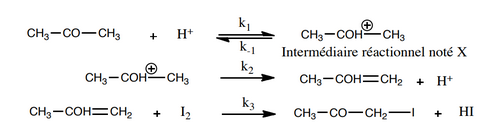
\includegraphics[scale = 0.7]{iodation_propanone.png}
	\caption{Mécanisme de l'iodation de la propanone.}
	\end{center}
\end{figure}
\begin{figure}[h!]
	\begin{center}
  		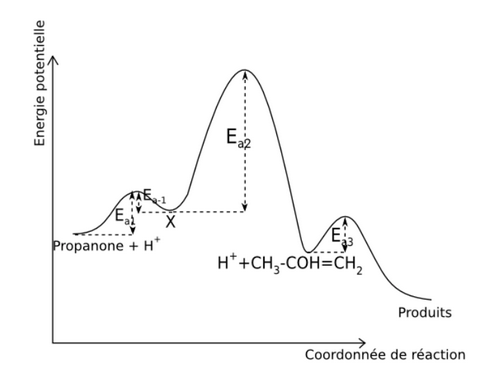
\includegraphics[scale = 0.6]{profil_reac.png}
	\caption{Profil réactionnel de l'iodation de la propanone.}
	\end{center}
\end{figure}

Chacune de ces étapes est un \textbf{acte élémentaire}, opération simple (rupture ou formation d'une liaison) impliquant une ou deux molécules sans intermédiaire réactionnel détectable. Le nombre de molécules impliquées dans un acte élémentaire constitue sa \textbf{molécularité} :
\begin{itemize}
	\item un acte élémentaire mono moléculaire correspond à une molécule qui se brise ou qui change 			de configuration;
	\item un acte élémentaire bimoléculaire correspond à une collision entre deux molécules;
	\item les collisions entre trois corps étant peu probables, les actes élémentaires sont 					généralement monomoléculaires ou bimoléculaires.
\end{itemize}
Il ne faut pas confondre la molécularité d'un acte (qui est une notion microscopique) et l'ordre d'une réaction. Pour un acte élémentaire, molécularité et ordre coïncident. Pour une réaction (caractérisée par son équation bilan), ce sont deux notions différentes.\\

Essayons de voir comment interpréter la loi de vitesse à la lumière de ce mécanisme :
\begin{itemize}
	\item Étape 1; \textbf{pré-équilibre rapide}, car l'étape 2 est très lente.
	\item Étape 2; étape lente, dite \textbf{étape cinétiquement déterminante}. C'est elle qui va avoir le plus d'influence sur la vitesse de réaction. Le diiode étant absent de cette étape, on comprend pourquoi il ne figure pas dans la loi de vitesse.
	Ces deux étapes constituent un \textbf{équilibre céto-énolique (tautomérie)}.
	\item Étape 3; étape facile, bien plus rapide que la précédente. L'énol formé lors de la seconde étape est consommé pratiquement dès qu'il produit. Il est donc raisonnable de considérer sa concentration comme faible et constante au cours de la réaction. Cette approximation est \textbf{l'approximation des régimes quasi-stationnaires}.
\end{itemize}

\textbf{La cinétique de la réaction est conditionnée par l'étape la plus lente}, c'est à dire la seconde (on parle d'étape cinétiquement limitante). Cette étape correspond à celle pour laquelle l'énergie d'activation à fournir est la plus importante.

\section*{Conclusion}
Nous avons vu dans cette leçon les notions de base de la cinétique chimique : 
\begin{itemize}
	\item on a défini la vitesse d'une réaction ainsi que la notion de loi de vitesse et d'ordre;
	\item on a mis en évidence quelques facteurs cinétiques (concentration, température) et leur influence à travers des lois empiriques, comme la loi d'Arrhénius;
	\item nous avons enfin discuté de plusieurs types de méthodes de suivi cinétique et mis en œuvre un suivi par spectrophotométrie pour illuster les méthodes intégrale et de dégénérescence de l'ordre.
\end{itemize}


\newpage
\section*{Annexes}
\subsection{Sur la réaction entre acide oxalique et permanganate de potassium}

Cette réaction est complexe : si le violet disparaît, cela ne signifie pas pour autant que la réaction est terminée : les produits finaux sont incolores ($\text{Mn}^{2+}$) mais la solution peut, pendant un certain temps, prendre une teinte jaune, signifiant le passage par un ou plusieurs intermédiaires réactionnels.

\subsection{Iodation de la propanone}

\textbf{Remarque n$\degree$1 :} la réaction a lieu avec $I_3^-$ et non avec $I_2$ (il y a un équilibre de complexation, très fortement déplacé en faveur de la formation du triiodure, mais vérifier).\\

\textbf{Remarque n$\degree$2 :} retrouver la loi de vitesse à partir du mécanisme :

\begin{equation}
	v_1 = k_1[H^+][\text{cétone}] \quad\text{et}\quad v_{-1} = k_{-1}[X]
\end{equation}
où $X$ désigne le premier intermédiaire réactionnel. Pour les deux étapes suivantes :
\begin{equation}
	v_2 = k_2 [X],
\end{equation}
\begin{equation}
	v_3 = k_3[I_2][\text{énol}].
\end{equation}

On définit la vitesse de réaction comme la vitesse de formation du produit :
\begin{equation}
	v_R \equiv \frac{d[I_2]}{dt} = v_3.
\end{equation}

Comme l'énol est lentement formé et rapidement consommé, on suppose que sa concentration reste faible et constante tout au long de la réaction (AEQS) :
\begin{equation}
	\frac{d}{dt}[\text{énol}] = v_2 - v_3 = 0 \quad\text{d'où}\quad v_2 = v_3.
\end{equation}
Ainsi
\begin{equation}
	v_R = k_2[X].
\end{equation}
Or, il y a pré-équilibre (étape 1 rapide, par rapport à l'étape 2), donc
\begin{equation}
	v_1 = v_{-1} \quad\text{d'où}\quad k_1[H^+][\text{cétone}] = k_{-1}[X],
\end{equation}
d'où d'une part la constante d'équilibre satisfaite, ce qui implique
\begin{equation}
	K\degree = \frac{k_1}{k_{-1}},
\end{equation}
et d'autre part
\begin{equation}
	[X] = [\text{cétone}][H^+],
\end{equation}
d'où la loi de vitesse
\begin{equation}
	\boxed{v_R = K\degree k_2\text{cétone}][H^+]}.
\end{equation}
\end{document}